\documentclass[a4paper,titlepage,10pt]{article}
\usepackage[margin=0.5in]{geometry}
\usepackage[spanish]{babel} % Le indicamos a LaTeX que vamos a escribir en espa�ol.
\usepackage[latin1]{inputenc} % Permite utilizar tildes y e�es normalmente
%\usepackage{framed}
\usepackage{caratula}
\usepackage{verbatim}
\setlength{\parindent}{0in}

\titulo{Trabajo Práctico 1\\Carpooling}
\fecha{23 / 09 / 2012}
\materia{Ingeniería De Software 1}
\grupo{Grupo 1}
\integrante{Browarnik, Martín}{04/10}{mibrowar0@gmail.com}
\integrante{Carreiro, Martín}{45/10}{martin301290@gmail.com}
\integrante{Kujawski, Kevin}{459/10}{kevinkuja@gmail.com}
\integrante{Ortiz de Zarate, Juan Manuel}{403/10}{jmanuoz@gmail.com}
\integrante{Soifer, Alexis}{25/10}{alex1879@gmail.com}
\begin{document} 

\maketitle

\section{Aclaraciones} %Decisiones tomadas por el grupo
Queremos aclarar que las flechas de las nubes O-refinamiento deberían salir de las flechas de los objetivos pero el programa que utilizamos no permitía esta opci\'on.

\section{Diagrama de Contexto} %Poner imagenes de contexto

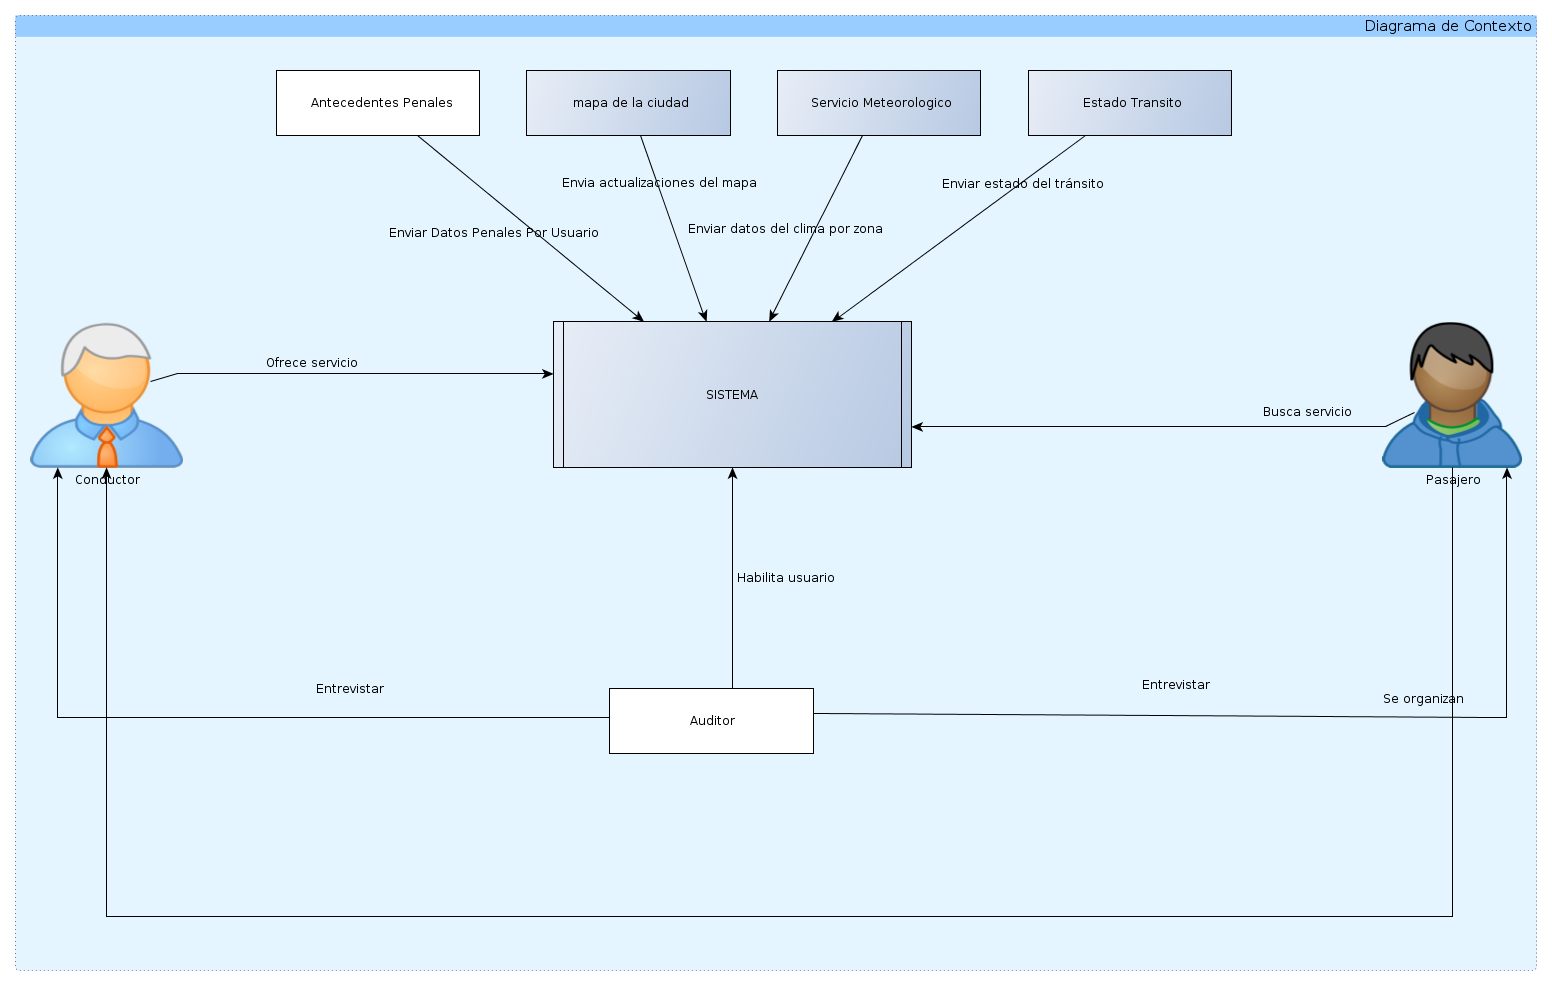
\includegraphics[height=7cm,width=17cm]{imagenes/contexto.png}

Los elementos en blanco pertenecen al O-refinamiento que se detallará en la secci\'on: Diagrama de Objetivos.

\newpage

\section{Diagrama de Objetivos} %Poner imagenes de objetivos

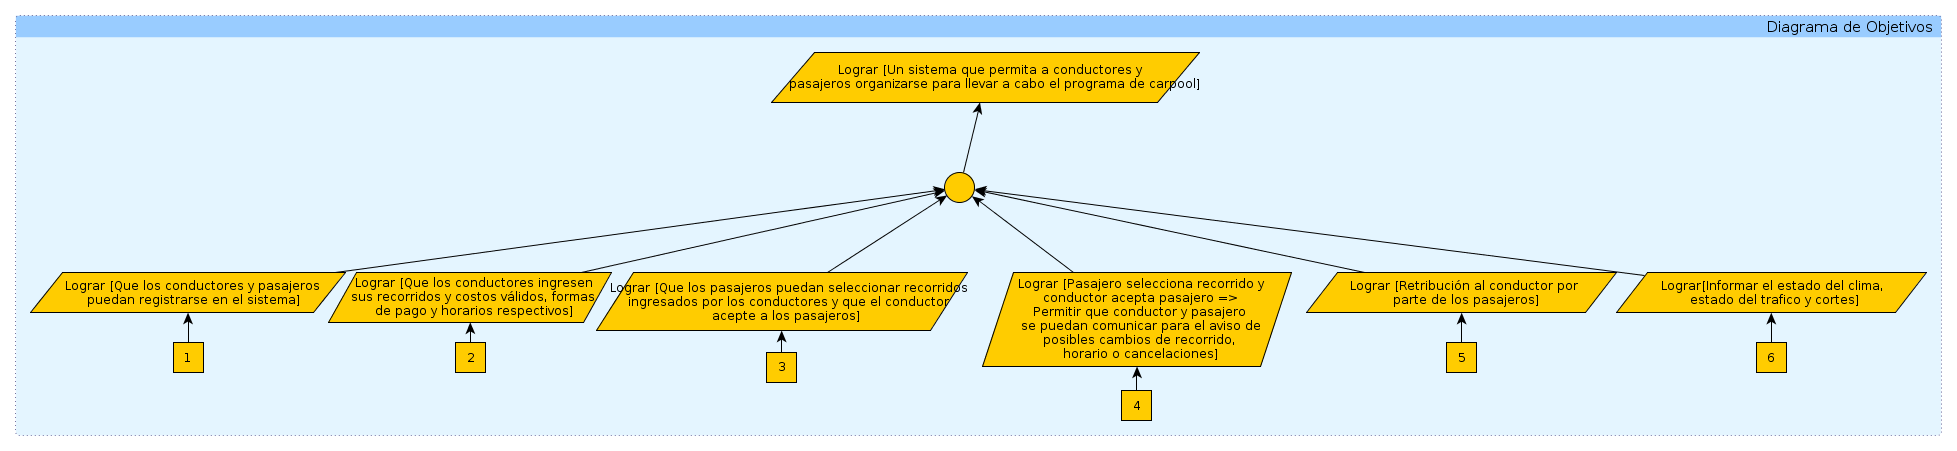
\includegraphics[height=7cm,width=19.5cm]{imagenes/root.png}

La organizaci\'on entre pasajeros y conductores para el sistema de Carpooling pretende que los usuarios interactuan en el sistema, en donde los conductores ingresarán sus recorridos (que serán validados), los 
cuales los pasajeros podrán filtrar y seleccionar entre estos, y que deberán ser aceptados por los mismos conductores, para luego proceder a la etapa de realizaci\'on y retribuci\'on del viaje. En base a las 
distintas alternativas planteadas, el sistema tendra una mayor confiabilidad, seguridad, facilidad de uso y anonimidad de los usuarios.

\subsection{Registrarse}
\begin{itemize}
\item En caso de tener el m\'odulo de antecedentes penales, el auditor se encargará de decidir la aprobaci\'on a los usuarios que al momento de registrarse cuenten con antecedentes, comunicandose con el mismo.
\end{itemize}
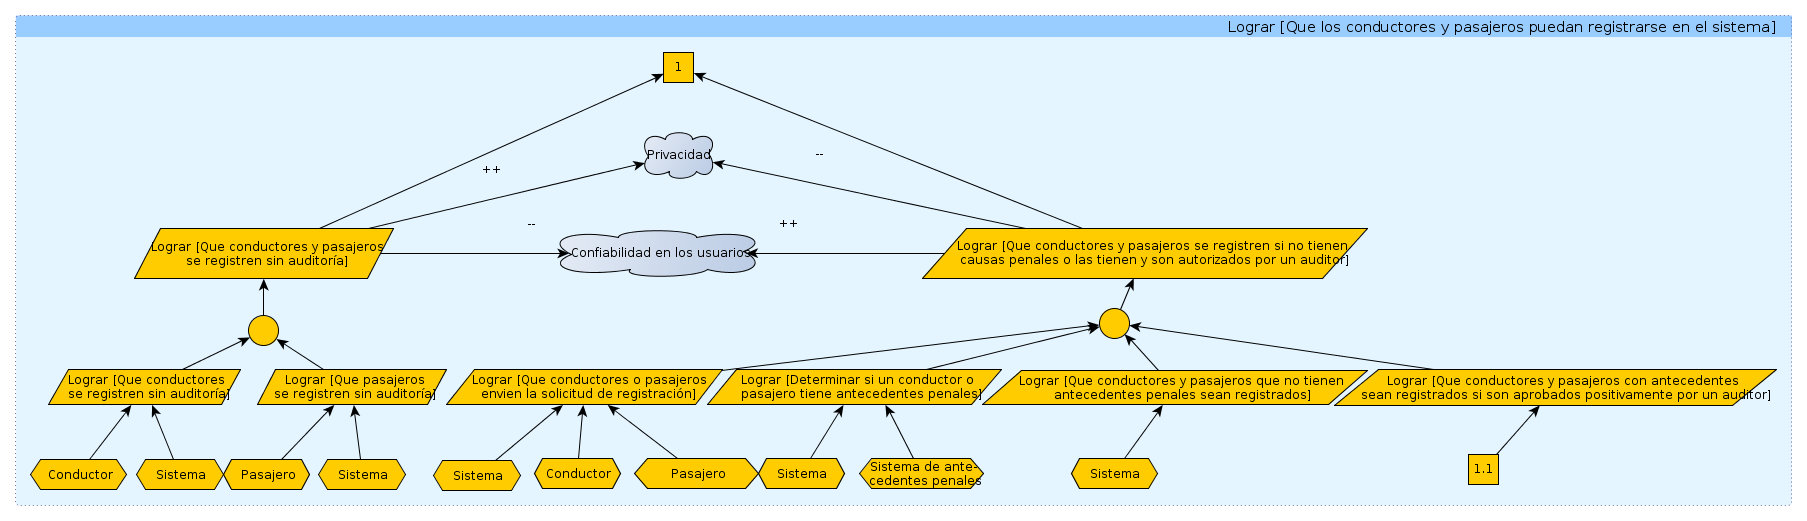
\includegraphics[height=7cm,width=19.5cm]{imagenes/Registrarse.png}
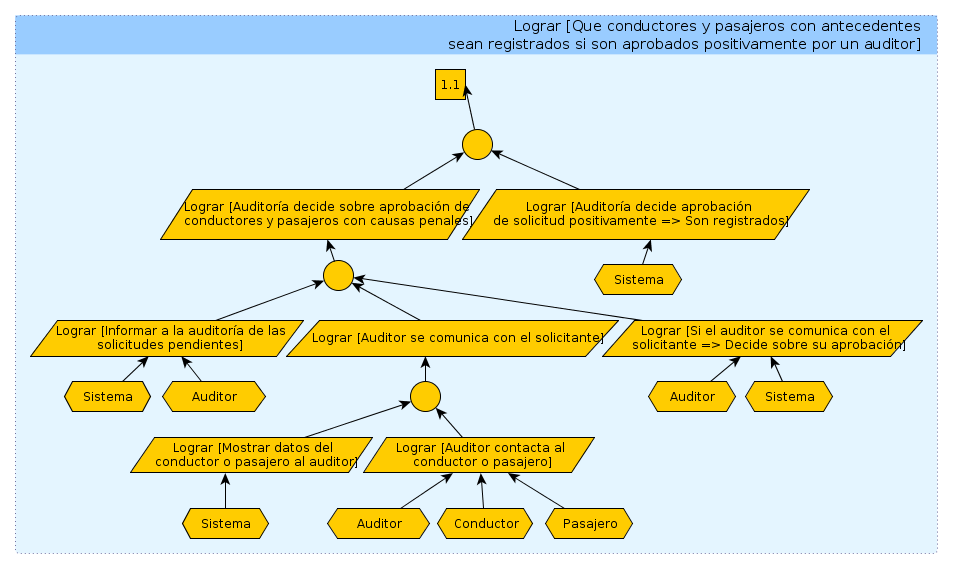
\includegraphics[height=7cm,width=19.5cm]{imagenes/Registrarsea.png}

\subsection{Ingresar Datos}
\begin{itemize}
\item Un recorrido es valido cuando nuestro sistema o el sistema externo de mapas realiza la correcta verificaci\'on de los datos ingresados por el conductor (calles, cruce de calles y alturas existentes)
\item El sistema validará los tiempos y costos del recorrido, es decir, el sistema cuenta con la informaci\'on necesaria sobre el tiempo de viaje (basandose en velocidades de calles del recorrido, trafico promedio en ese horario) y los costos del mismo (precio del combustible, peajes, mantenimiento del vehiculo) para establecer un rango de valores posibles para estos.
\end{itemize}
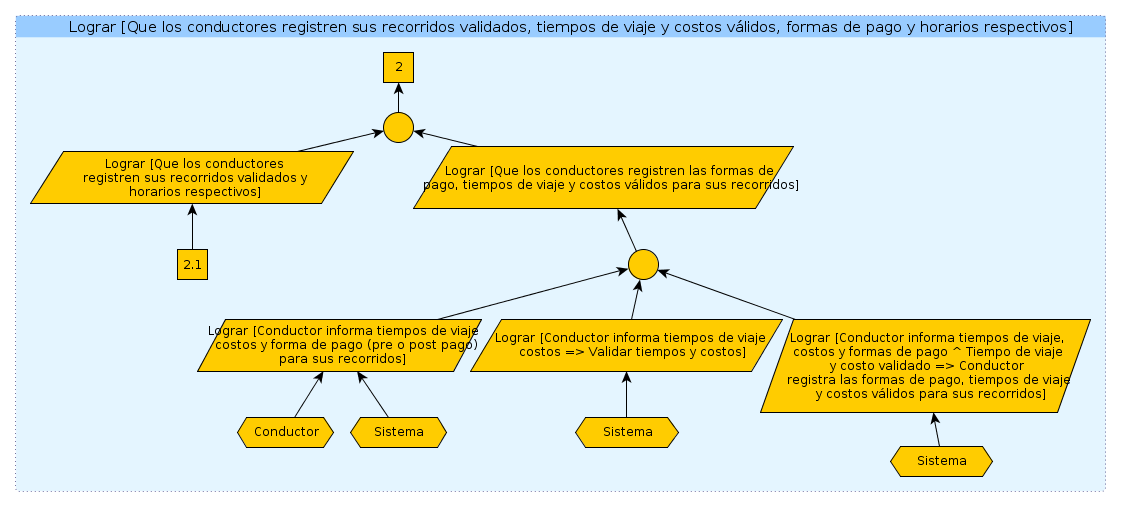
\includegraphics[height=7cm,width=19.5cm]{imagenes/Ingresenrecorridos.png}
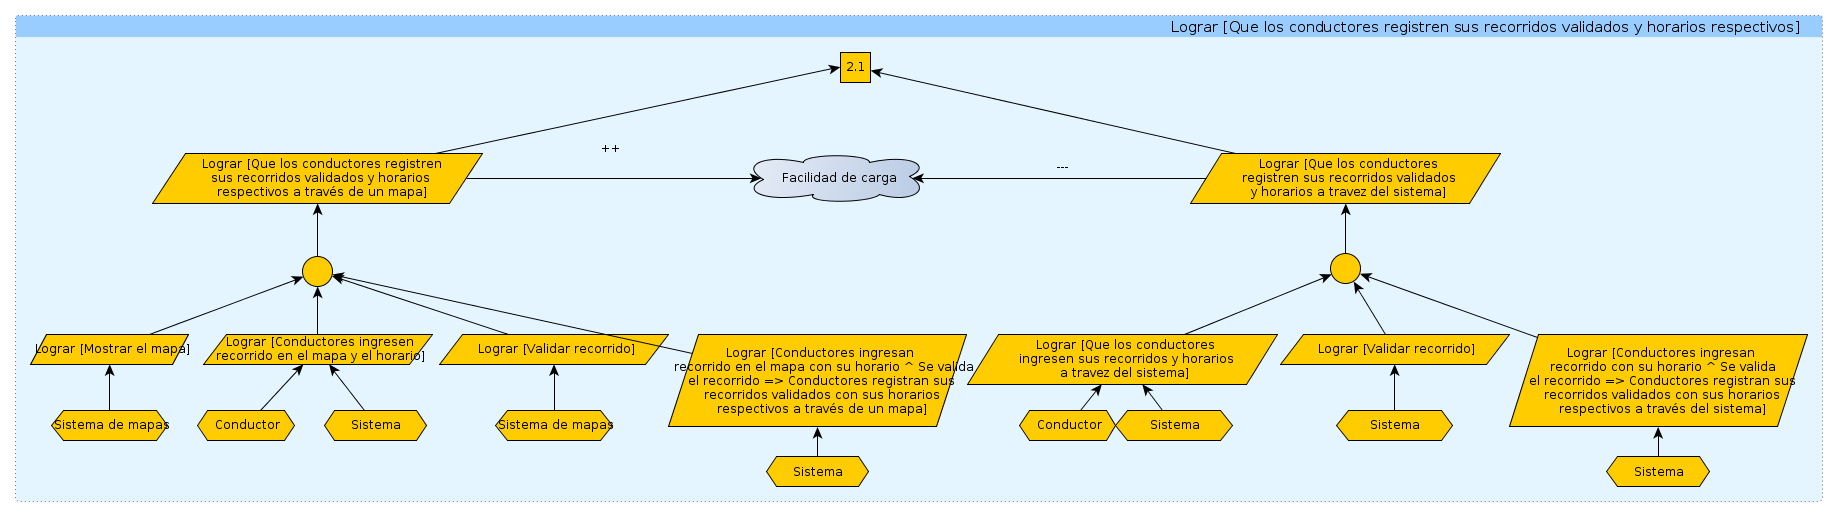
\includegraphics[height=7cm,width=19.5cm]{imagenes/Ingresenrecorridosa.png}

\newpage
\subsection{Seleccionar Recorrido y Aceptar}
\begin{itemize}
\item El sistema sabe si el pasajero y conductor tuvieron acuerdo ya que en la base de datos se guarda la seleccion del pasajero y luego la aceptaci\'on del conductor.
\item Cuando un conductor califica al pasajero esta informaci\'on se guarda en la base de datos
\item El conductor acepta al pasajero a traves de una pantalla en la que visualiza todas las solicitudas para los viajes ingresados por \'el.
\item Un viaje se considera organizado cuando el conductor acepta al pasajero en su recorrido
\end{itemize}
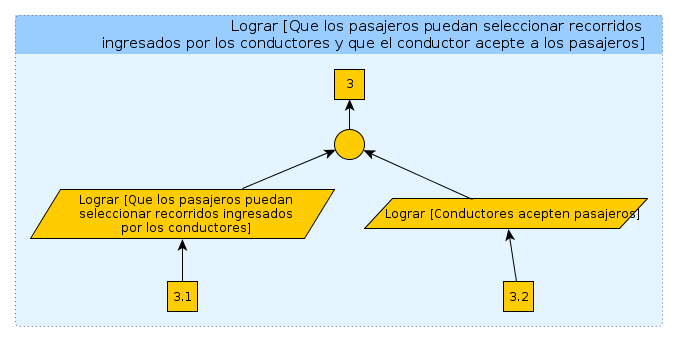
\includegraphics[height=7cm,width=19.5cm]{imagenes/Mostrar.png}
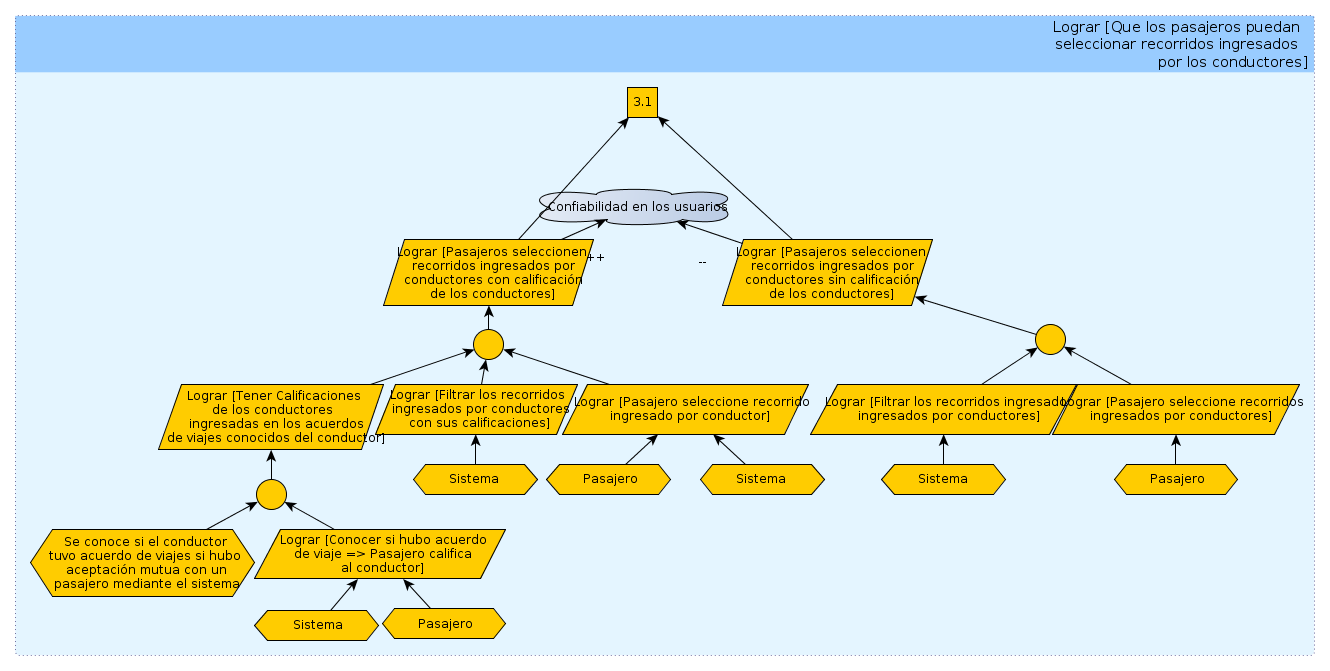
\includegraphics[height=7cm,width=19.5cm]{imagenes/Mostrara.png}
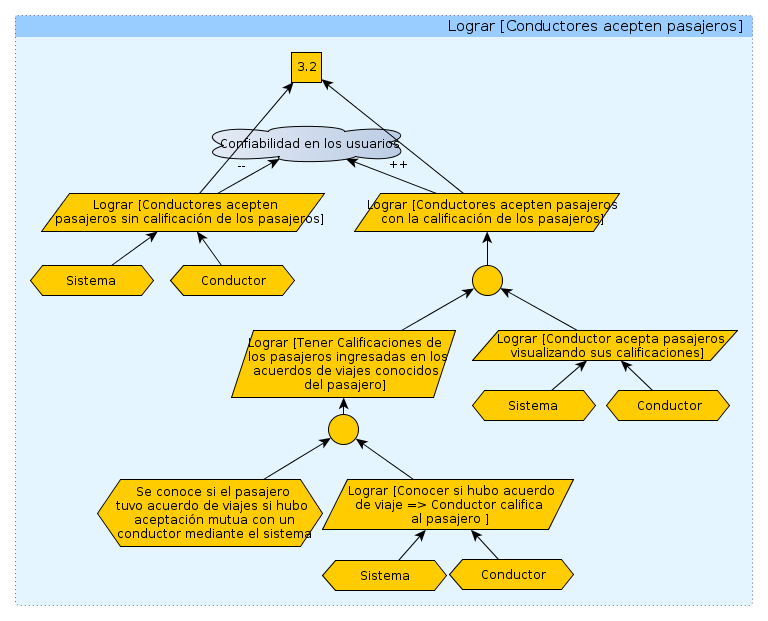
\includegraphics[height=7cm,width=19.5cm]{imagenes/Mostrarb.png}

\subsection{Comunicaci\'on}
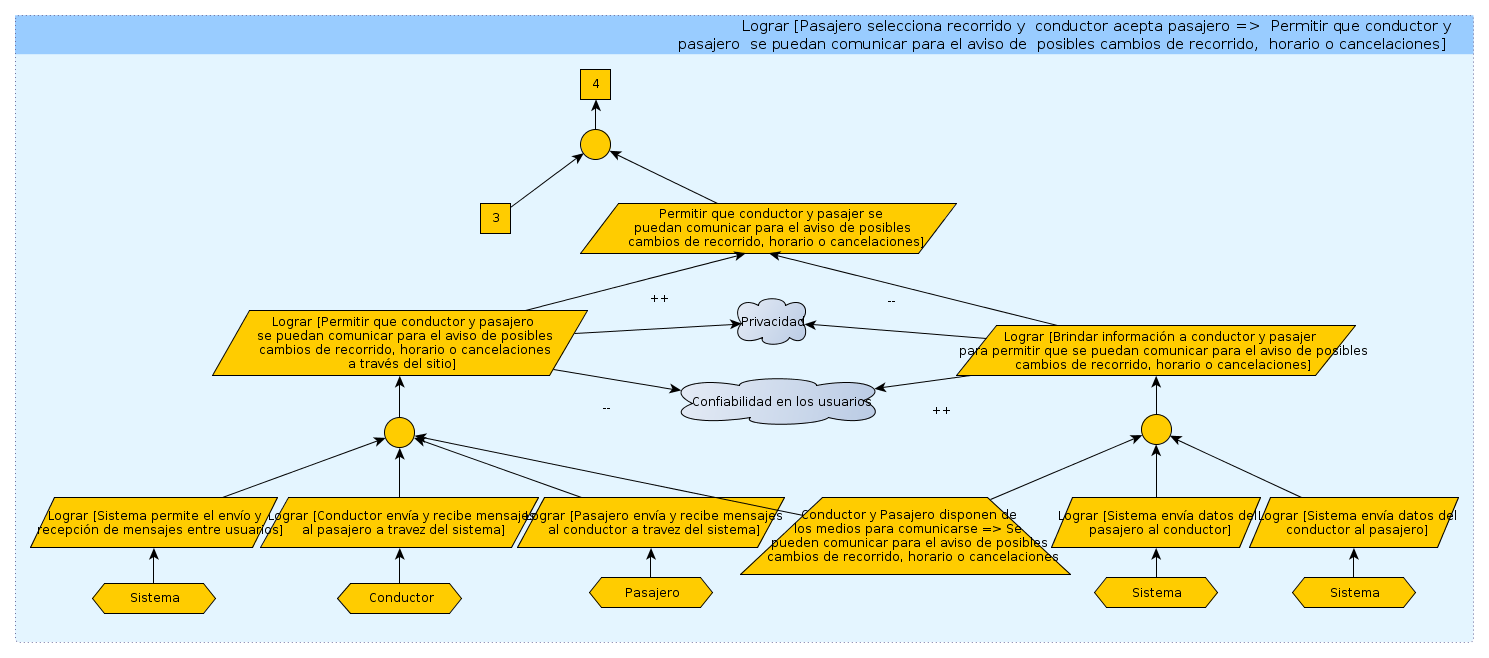
\includegraphics[height=7cm,width=19.5cm]{imagenes/Comunicacion.png}

\subsection{Retribuci\'on}
\begin{itemize}
\item El sistema sabe si el pasajero y conductor tienen acordado un viaje entre ellos
\item En caso de pago diferido, el pasajero deposita su pago en el sistema a traves de una pantalla seleccionando alguna de las alternativas de pago, y luego de que se produzca el sistema lo almacenara en la base de datos, "congelando" el deposito hasta que se informe si se produzco el viaje
\item En caso de pago diferido, pasada la fecha del viaje, los pasajeros y el conductor informarán al sistema (a traves de una pantalla con todos sus viajes organizados) si el viaje se realizo para que de cumplirse este, el pago $"$congelado$"$ realizado anteriormente por el pasajero se le acredite al conductor. En caso de no realizarse el viaje el conductor también recibira el pago, a no ser que no se haya sido su falta.
\end{itemize}
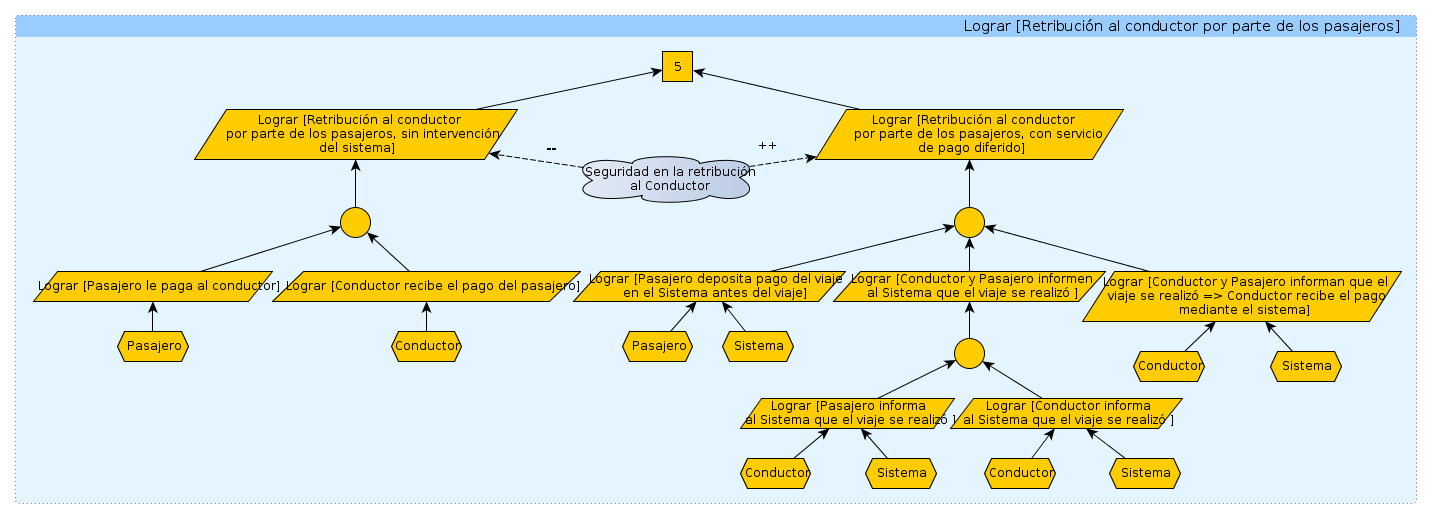
\includegraphics[height=7cm,width=19.5cm]{imagenes/Retribucion.png}

\subsection{Informaci\'on}
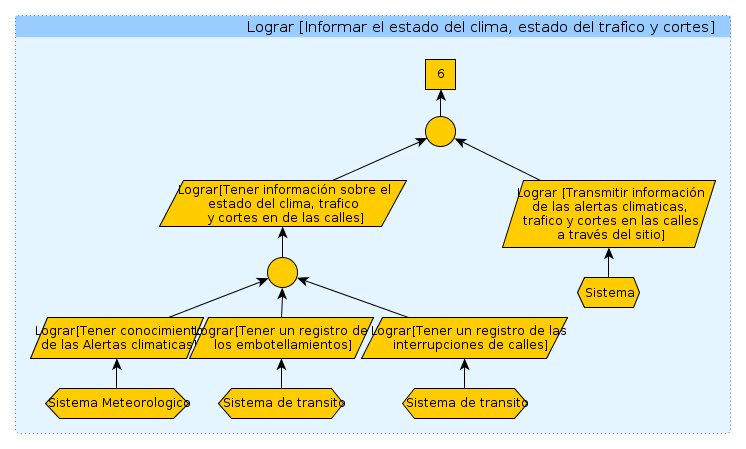
\includegraphics[height=7cm,width=19.5cm]{imagenes/InformacionDelClimayViajes.png}



\newpage

\section{Escenarios} %Escribir los escenarios
Aqu� detallaremos algunos de los posibles escenarios del sistema de Carpooling

\subsection{Escenario 1: Conductor del programa de Carpooling}
Javier Baez, es un trabajador de una empresa que queda en el centro de cambodia, todos los dias se levanta muy temprano para ir a trabajar
porque lamentablemente la cantidad de autos que van hacia el mismo lugar es muy alta, utiliza el mismo recorrido todos los dias truene o salga el sol.
Es en uno de sus viajes al trabajo observa que el conductor del auto de su costado es un compa\~nero de trabajo, Alberto, y que estan junto a el otras 3 personas que nunca habia visto.
Cuando llega al trabajo, lo ve sin ninguna compa\~nia y por curiosidad le pregunta quienes eran sus acompa\~nantes, este responde que los conoci\'o a travez del programa de carpooling promocionado por el 
gobierno, sin entender de que se trata, Javier le pregunta la razon por la que utiliza el programa de carpooling y si no le asustaba que se suban extra\~nos en su auto, este responde que de esa manera 
disminuyen la cantidad de automoviles en la calle lo que afecta directamente al trafico que hay en su recorrido al trabajo y que el sistema le permite aceptar o no al solicitante que va a subirse a su 
automovil. Sorprendido por la respuesta, Javier se da cuenta de que existe una solucion a los problemas de trafico que tiene que lidiar todos los dias y decide entrar al sitio del gobierno para conocer 
mejor el funcionamiento del carpool, es asi como cuando llega a su oficina descubre que el sistema planteado le permite seleccionar quienes viajarian con el, de manera que el se sienta seguro, y que muchas 
otras personas conocidas ya participan del programa, ademas, advierte algo que su compa\~nero no le habia informado, no solamente el sistema le permitiria reducir el tiempo en realizar su recorrido sino que 
tambi\'en los usuarios le pagarian a el por transportarlos lo que reduciria una parte de sus gastos diarios. Entusiasmado, rapidamente se registra en el programa como conductor, ingresa su recorrido y costo 
y vuelve a trabajar. Al finalizar su horario de trabajo, ingresa al sitio para verificar si alg\'un pasajero desea volver con el y para su sorpresa son 5 los solicitantes, de ah� Javier elige a 3, se 
comunica con ellos a travez del sistema, se aceptan mutuamente y establecen la forma de pago. Todo funciona a la perfecci\'on y Javier vuelve muy contento a su casa.

\subsection{Escenario 2: Pasajero del programa de Carpooling}
Al llegar a su casa, Javier le comenta a su mujer, Marina, de su descubrimiento, ella, como usuario del transporte publico se ve muy interesada en algo que le permita evitar las largas horas de viaje parada lo que le resulta muy incomodo y molesto para ir a trabajar, es asi que decide investigar un poco de que se trata el sistema.
Luego de registrarse descubre en el que existen muchos Conductores que realizan viajes parecidos al de ella y con un costo que ella considera correcto, entonces decide enviar la solicitud a un conductor, est\'a se pone en contacto con ella y se ponen de acuerdo para ir juntos al dia siguiente.
Al dia siguiente, el dia del viaje, Marina decide entrar al sistema para abonar el viaje y advierte que la ruta acordada estaba intervenida por unos empleados en huelga, es asi que se pone en contacto con el Conductor y deciden modificar el recorrido, en ese mismo momento el conductor advierte al resto de los pasajeros del cambio de recorrido y el viaje se realiza de forma correcta y sin inconvenientes de trafico.
Luego de este viaje, Marina se siente muy satisfecha con el sistema y se lo comenta a todos sus compa\~neros de trabajo.

\end{document} %Termine!
